\chapter{Results and Discussion}
\section{DE Convergence Analysis}
Figure~\ref{fig:convergence} shows the saved best-so-far development RMSE histories for both search methods. The horizontal axis counts objective evaluations, including initialization. Curves indicate optimization progress on the fixed development folds, not test accuracy. A lower validation endpoint does not guarantee a lower holdout error on a particular seed.
\begin{figure}[htbp]\centering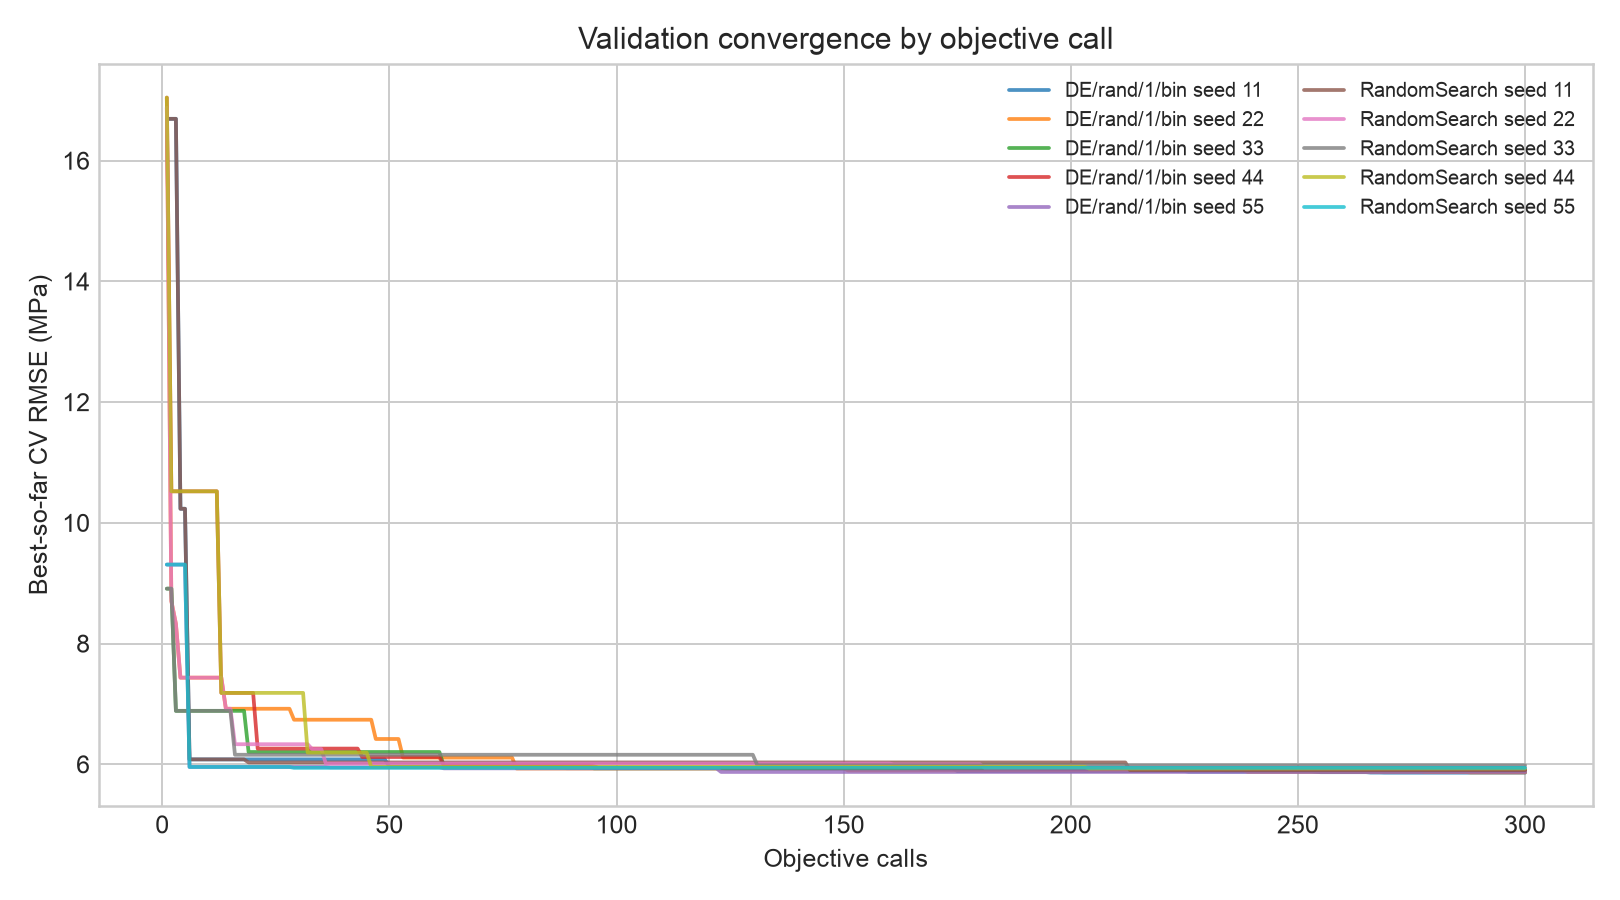
\includegraphics[width=\textwidth]{assets/convergence.png}\caption{Development validation convergence at equal candidate budgets.}\label{fig:convergence}\end{figure}
Figure~\ref{fig:searchspace} pools the 1{,}500 candidates each method evaluated over the five seeds. Random Search samples the box uniformly, so most of its calls fall in poor regions (large CV RMSE). DE concentrates its later calls in a narrow band of large $C$ and moderate $\gamma$, and many DE candidates sit on the upper bound $\log_{10}C=4$ because of coordinate clipping. Concentration does not translate into a meaningful holdout gain here: the good region is wide and flat, so uniform sampling with 300 calls also lands in it.
\begin{figure}[htbp]\centering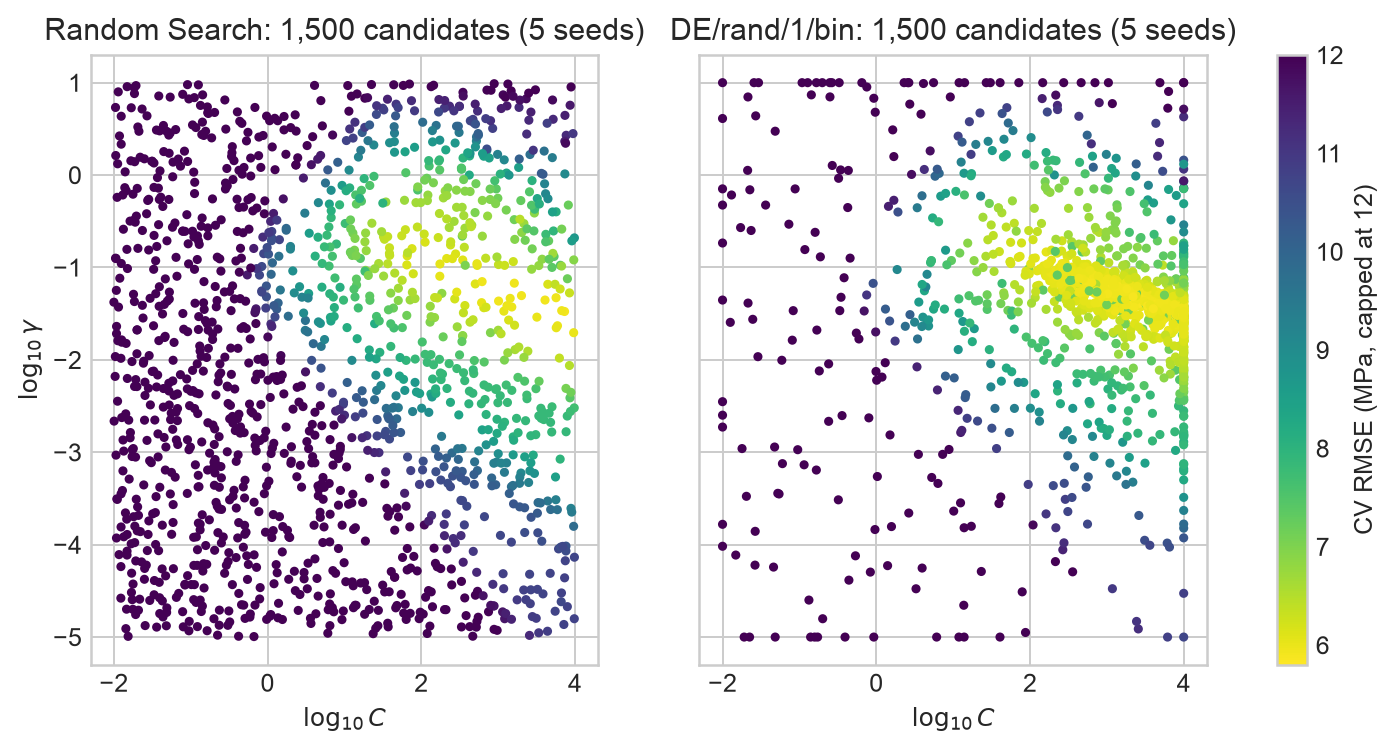
\includegraphics[width=\textwidth]{assets/search_space.png}\caption{Candidates evaluated by Random Search and DE, coloured by development CV RMSE (capped at 12 MPa).}\label{fig:searchspace}\end{figure}
\section{Optimal Hyperparameter Configuration}
The best observed validation-selected demonstration is DE seed 11, with CV RMSE 5.8601 MPa. The decoded values are $C=1462.1749$, $\gamma=0.0573784$ and $\epsilon=1.3447436$. ``Optimal'' refers to the best observed candidate in this finite search; no proof of a global optimum is implied. Its holdout RMSE is 6.3712 MPa, MAE 4.2896 MPa and $R^2=0.8244$.
\section{Prediction Performance}
Table~\ref{tab:metrics} gives the holdout comparison. Tuned values are mean $\pm$ sample SD over five optimizer seeds. Default SVR is one fixed configuration. Every model is evaluated on the same 204 holdout observations.
\begin{table}[htbp]\centering\caption{Holdout results; tuned values are five-seed mean $\pm$ sample SD.}\label{tab:metrics}\begin{tabularx}{\textwidth}{Xlll}\toprule Model&RMSE (MPa)&MAE (MPa)&$R^2$\\\midrule
Default RBF-SVR & 9.9069 & 7.8854 & 0.5755\\
Random Search--SVR & $6.2328\pm0.1194$ & $4.3502\pm0.0253$ & $0.8319\pm0.0064$\\
DE--SVR & $6.2250\pm0.1104$ & $4.3143\pm0.0526$ & $0.8324\pm0.0060$\\\bottomrule\end{tabularx}\end{table}
DE improves mean RMSE relative to default by approximately 37.2\%. Its 0.0078 MPa advantage over Random Search is approximately 0.125\% of Random Search RMSE. Both tuned methods therefore provide essentially equivalent holdout performance within this experiment.
\begin{figure}[htbp]\centering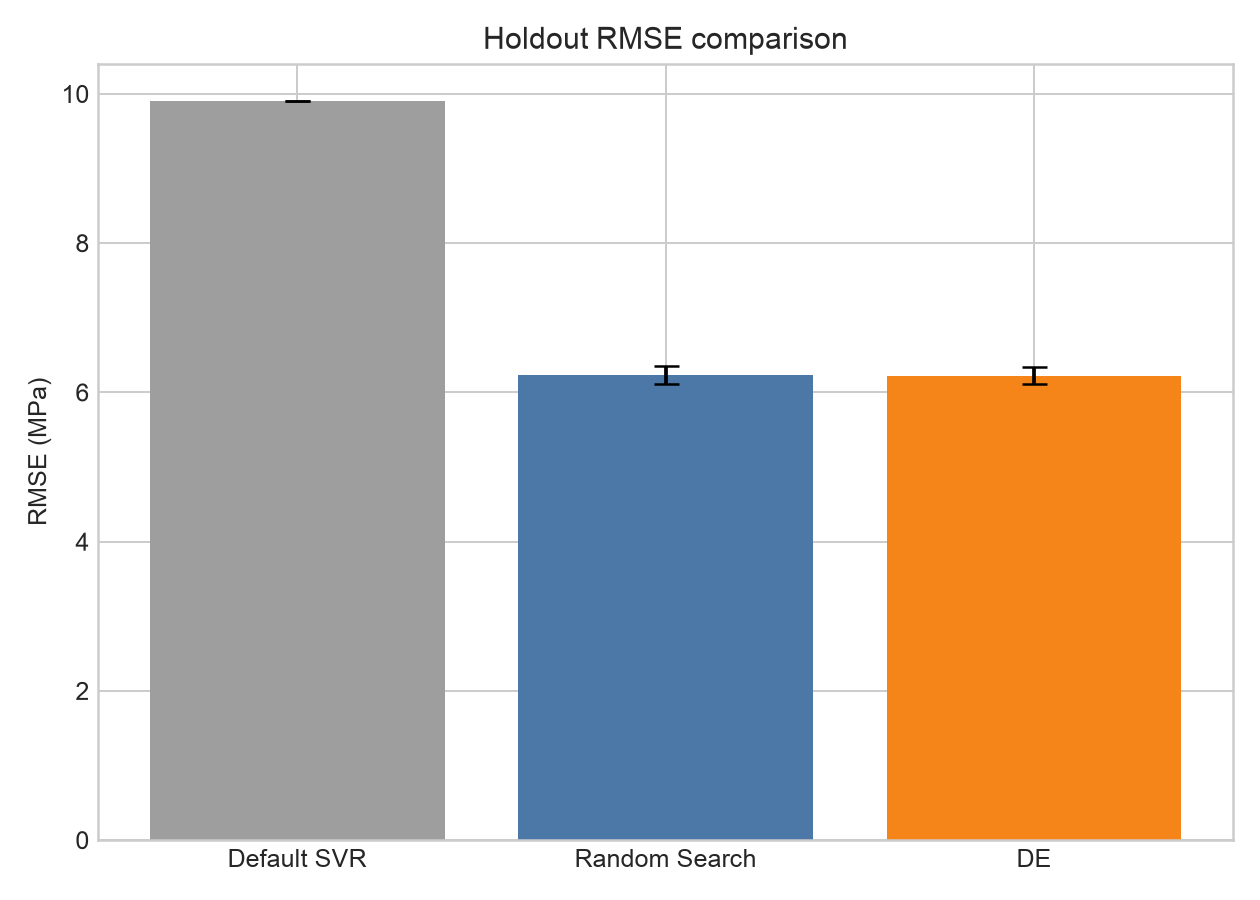
\includegraphics[width=0.7\textwidth]{assets/holdout_rmse_comparison.png}\caption{Holdout RMSE: default SVR and five-seed tuned-model aggregates. Error bars describe optimizer-seed SD.}\label{fig:comparison}\end{figure}
\section{Temporal Performance Analysis}
Temporal regime analysis is not applicable to this cross-sectional tabular dataset. Curing age is a predictor rather than a time-ordering rule for samples. No chronological regime or rolling-window result was produced. Age-stratified error analysis could be evaluated in future work under a declared protocol.
\section{Comparison with Baseline Models}
The default model's RMSE of 9.9069 MPa and $R^2$ of 0.5755 show the limits of its untuned settings on this partition. Random Search reaches $R^2=0.8319\pm0.0064$ and DE reaches $0.8324\pm0.0060$. The agreement of tuned holdout results is more substantial than their difference. A strong random baseline is necessary to avoid attributing every tuning gain to DE.
\section{Hyperparameter Importance Analysis}
The saved search histories contain candidate values and fitness scores, but the project did not perform an independent hyperparameter-importance experiment. Search correlations are influenced by the sampling strategy and interactions among parameters. They would not establish causal importance. No importance ranking is claimed.
\section{Feature Importance Results}
No permutation-importance, SHAP or ablation study was performed. An RBF-SVR does not supply directly interpretable linear feature coefficients. The report therefore does not invent an ingredient ranking. Any future explanation study should use development data for design decisions and state the uncertainty of its interpretation.
\section{Error Analysis}
Figure~\ref{fig:residuals} presents predictions and residuals for the validation-selected demonstration, DE seed 11. All holdout measurements remain in the figure, including large errors. No post-hoc removal was performed. The plot shows the behavior of this selected configuration; it is not an average of predictions from five models.
\begin{figure}[htbp]\centering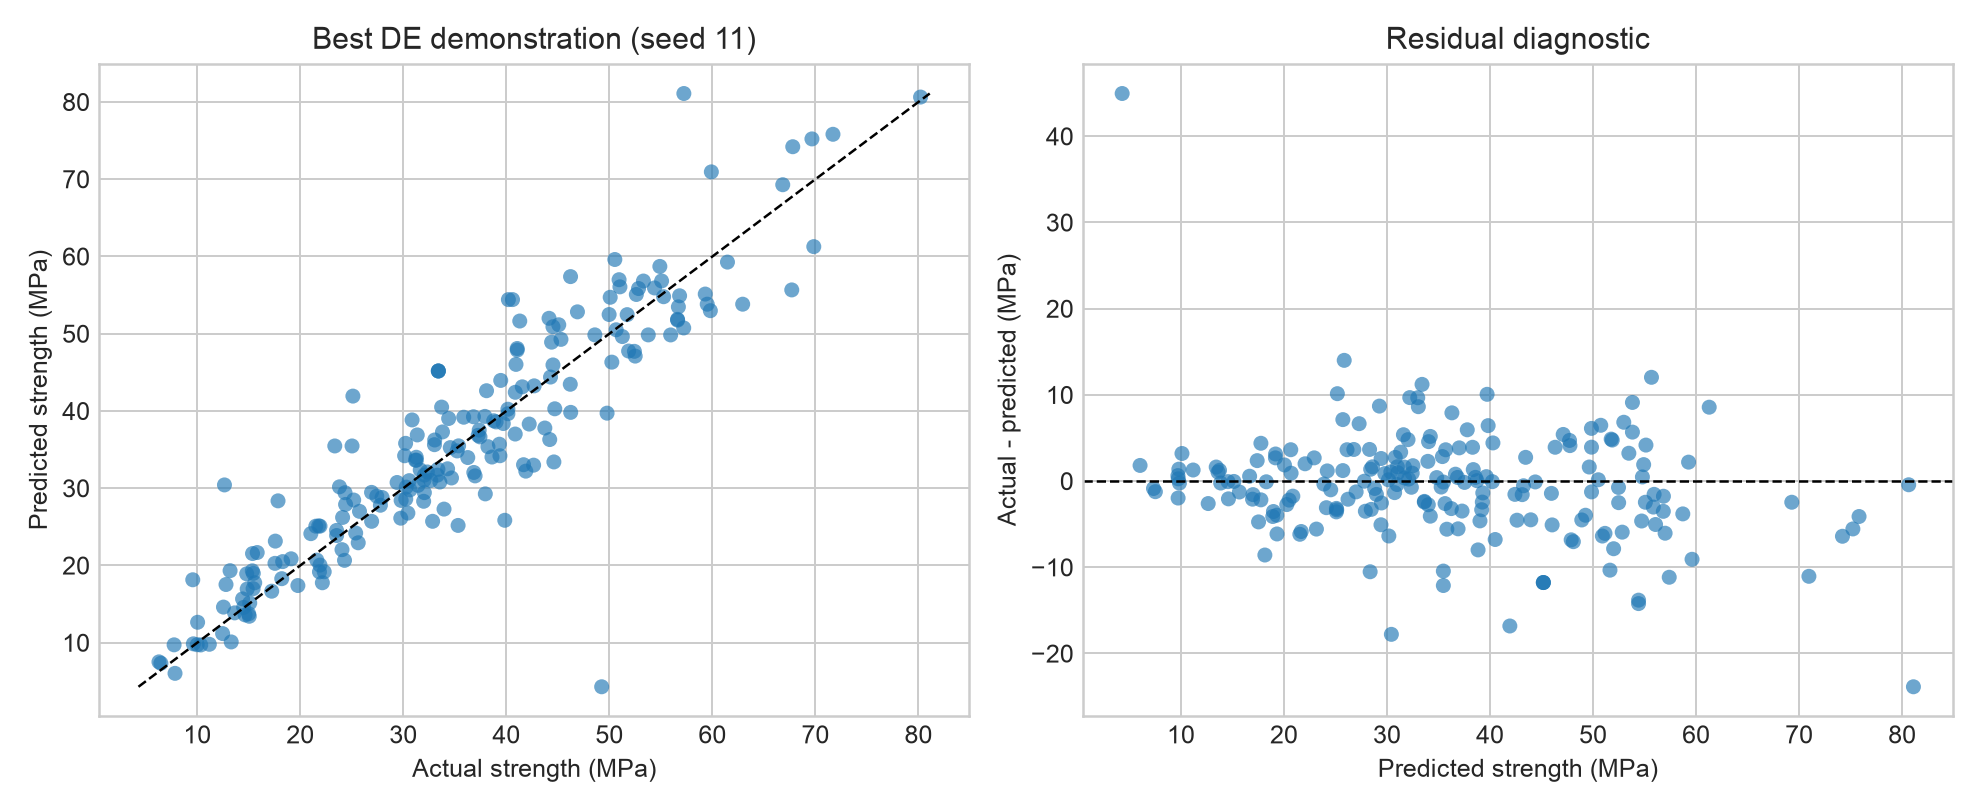
\includegraphics[width=\textwidth]{assets/prediction_residuals.png}\caption{Predictions and residuals for the validation-selected demonstration, DE seed 11.}\label{fig:residuals}\end{figure}
Residual patterns are descriptive. A plot alone does not establish homoscedasticity, normality or absence of bias. The study reports no Breusch--Pagan test or other unsupported inferential diagnostic.
\section{Computational Performance}
The complete search budget is 1,500 candidate evaluations per method, each scored on five development folds. Every attempted candidate is counted. The demonstration's saved final development refit takes 0.4194 seconds in the original experiment environment; this excludes search time and is not an end-to-end runtime claim. The repository retains per-call timing histories for further inspection.
\section{Robustness Analysis}
Table~\ref{tab:perseed} lists the holdout metrics of every predefined validation-selected run.

\begin{table}[htbp]\centering\caption{All ten predefined validation-selected runs, evaluated on the same holdout.}\label{tab:perseed}\begin{tabularx}{\textwidth}{lCCCC}\toprule Method&Seed&RMSE (MPa)&MAE (MPa)&$R^2$\\\midrule
DE & 11 & 6.3712 & 4.2896 & 0.8244\\
DE & 22 & 6.1675 & 4.2513 & 0.8355\\
DE & 33 & 6.0830 & 4.3471 & 0.8400\\
DE & 44 & 6.2871 & 4.3860 & 0.8290\\
DE & 55 & 6.2163 & 4.2974 & 0.8329\\\midrule
Random Search & 11 & 6.3884 & 4.3422 & 0.8235\\
Random Search & 22 & 6.0950 & 4.3603 & 0.8393\\
Random Search & 33 & 6.1456 & 4.3827 & 0.8367\\
Random Search & 44 & 6.3112 & 4.3520 & 0.8277\\
Random Search & 55 & 6.2238 & 4.3138 & 0.8325\\\bottomrule\end{tabularx}\end{table}

Across seeds, DE holdout RMSE SD is 0.1104 MPa and Random Search SD is 0.1194 MPa. These values quantify optimization variability on this one holdout. They do not measure robustness to a different dataset, partition, measurement process or concrete source.

The corrected learning curve (Figure~\ref{fig:learning}) uses three development-only folds. Within each fold, training subsets are nested samples of complete groups at fractions 0.25, 0.50, 0.75 and 1.00. Parameters remain fixed; there is no retuning or holdout access. Mean validation RMSE declines from 8.3838 to 5.9784 MPa while mean training RMSE rises from 2.7596 to 3.7728 MPa. The remaining gap suggests that the fitted model has lower error on its training subsets than on validation groups.
\begin{figure}[H]\centering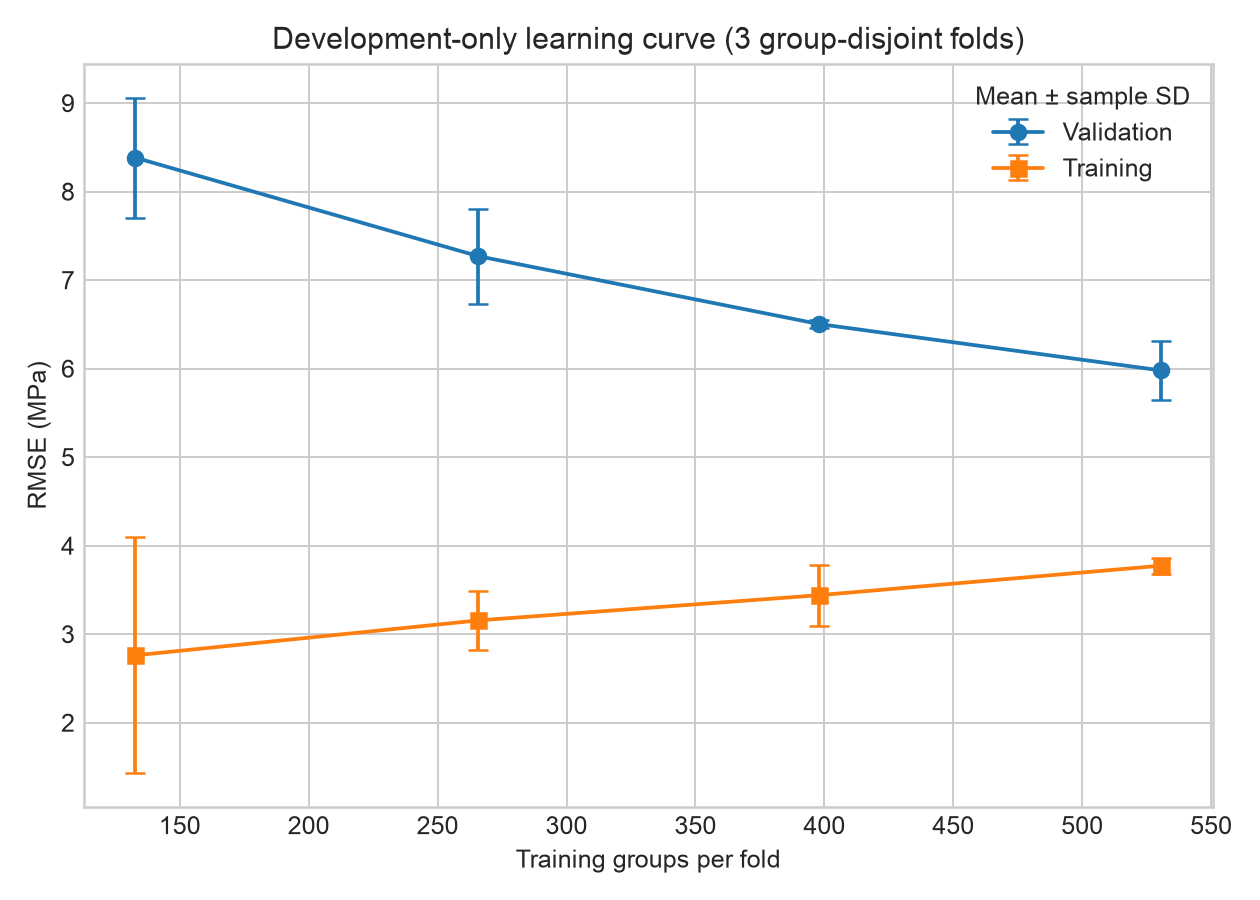
\includegraphics[width=0.78\textwidth]{assets/learning_curve.png}\caption{Three-fold development diagnostic with nested whole-group samples and fixed demonstration parameters.}\label{fig:learning}\end{figure}
These diagnostic values do not replace the five-fold search objective or provide an additional independent generalization estimate.
\section{Discussion}
The most defensible finding is that configuration matters: both tuned methods materially improve default SVR. DE finds slightly lower mean development RMSE, but the advantage almost disappears on holdout. This illustrates why validation optimization progress and independent predictive performance must be reported separately.

The scope of the frozen experiment remains one dataset, one model, one fixed partition and five optimizer seeds; Extension~2 (Section~\ref{sec:extension2}) later added five further splits. Historical holdout exposure, finite budgets and environment differences limit interpretation. The evidence supports a reproducible comparison within that scope, rather than a general claim that evolutionary methods outperform random search.
\section{Extension: Log-Age Input Representation}\label{sec:extension}
\subsection{Motivation and protocol}
After the frozen results were complete, a development-only probe (five saved CV folds, no holdout access, nothing saved) suggested that the optimizer was not the limiting factor: replacing age with $\ln(\text{age})$ lowered mean CV RMSE from about 5.85 to 4.97 MPa. This extension tests that observation under the full matched protocol, which was written and committed before any extension search was run (\texttt{docs/protocol-extension.md}). The data splits, folds, fold-local scaling, bounds, 300-call budget and seeds 11--55 are unchanged. The only change is a row-wise, deterministic input transform applied before scaling, so nothing is fitted on holdout data. Default SVR, Random Search and DE/rand/1/bin all use the same ln(age) representation. The frozen raw-feature results are reused unchanged for comparison and are not rerun.

Two disclosures apply. First, ln(age) was chosen because of the development probe, so it is a motivated choice rather than a blind one. Second, the holdout had already been inspected in Stage 1; selection in the extension still used only development CV RMSE, and the 25 candidates were frozen before a single holdout evaluation.
\subsection{Results}
Table~\ref{tab:extension} and Figure~\ref{fig:representation} give the comparison. With ln(age), default SVR improves from 9.9069 to 7.4780 MPa holdout RMSE, Random Search from 6.2328 to $4.9700\pm0.2656$ MPa and DE from 6.2250 to $4.8402\pm0.1039$ MPa, a reduction of about 22.2\% for DE relative to frozen DE and about 51\% relative to default SVR on raw features. The representation therefore accounts for most of the additional gain; tuning on top of it still improves default SVR by a large margin (7.4780 to 4.8402 MPa).

DE's mean holdout RMSE is 0.130 MPa (about 2.6\%) below Random Search on ln(age), and its seed-to-seed SD is smaller (0.1039 versus 0.2656 MPa). Validation RMSE shows the same ordering (4.9670 versus 5.0171 MPa). This is a small difference across five seeds on one partition and is not tested for significance, so it is reported as an observed tendency, not as established superiority.
\begin{table}[htbp]\centering\caption[Extension results]{Raw features (frozen) versus ln(age) features. Tuned values are five-seed mean $\pm$ sample SD on the same 204 holdout rows; default rows show the single five-fold CV mean and the single holdout score.}\label{tab:extension}\footnotesize\setlength{\tabcolsep}{2pt}\begin{tabularx}{\textwidth}{lCCCC}\toprule Model&Validation RMSE&Holdout RMSE&Holdout MAE&Holdout $R^2$\\\midrule
\multicolumn{5}{l}{\textit{Raw features (frozen results)}}\\
Default SVR & 10.3140 & 9.9069 & 7.8854 & 0.5755\\
Random Search & \mbox{$5.9399\pm0.0287$} & \mbox{$6.2328\pm0.1194$} & \mbox{$4.3502\pm0.0253$} & \mbox{$0.8319\pm0.0064$}\\
DE rand/1/bin & \mbox{$5.8797\pm0.0198$} & \mbox{$6.2250\pm0.1104$} & \mbox{$4.3143\pm0.0526$} & \mbox{$0.8324\pm0.0060$}\\
\midrule\multicolumn{5}{l}{\textit{ln(age) features (extension)}}\\
Default SVR & 8.4000 & 7.4780 & 5.6198 & 0.7581\\
Random Search & \mbox{$5.0171\pm0.0687$} & \mbox{$4.9700\pm0.2656$} & \mbox{$3.3607\pm0.0773$} & \mbox{$0.8929\pm0.0116$}\\
DE rand/1/bin & \mbox{$4.9670\pm0.0284$} & \mbox{$4.8402\pm0.1039$} & \mbox{$3.2623\pm0.0576$} & \mbox{$0.8987\pm0.0044$}\\
\midrule\multicolumn{5}{l}{\textit{DE ablations on ln(age) (same 300-call budget)}}\\
DE current-to-best/1/bin & \mbox{$4.9028\pm0.0701$} & \mbox{$4.8363\pm0.0582$} & \mbox{$3.3322\pm0.0724$} & \mbox{$0.8988\pm0.0024$}\\
jDE & \mbox{$4.8976\pm0.0234$} & \mbox{$4.8890\pm0.0820$} & \mbox{$3.3221\pm0.0633$} & \mbox{$0.8966\pm0.0035$}\\
DE rand/1/bin + water ratios & \mbox{$4.9611\pm0.0120$} & \mbox{$4.7849\pm0.0630$} & \mbox{$3.2696\pm0.0628$} & \mbox{$0.9010\pm0.0026$}\\
\bottomrule\end{tabularx}\end{table}

\begin{figure}[htbp]\centering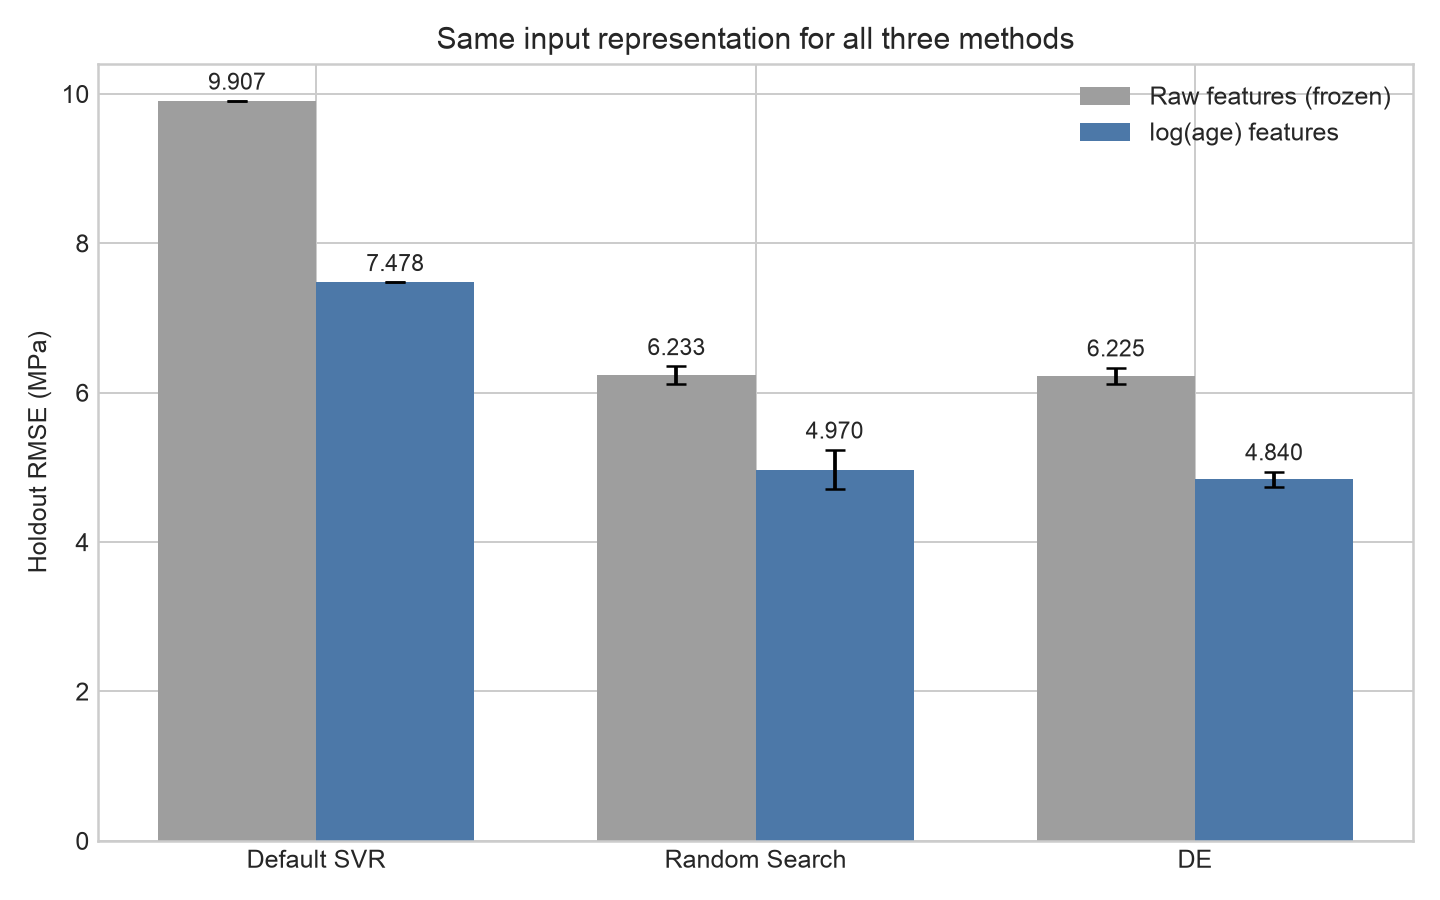
\includegraphics[width=0.8\textwidth]{assets/representation_comparison.png}\caption{Holdout RMSE for default SVR, Random Search and DE with raw features (frozen) and ln(age) features. Error bars are optimizer-seed SD.}\label{fig:representation}\end{figure}
\subsection{DE variant and feature ablations}
Figure~\ref{fig:variants} compares DE/rand/1/bin with DE/current-to-best/1/bin and with jDE~\cite{jde}, which adapts $F$ and $CR$ per individual, under the same budget. Holdout RMSE is 4.8402, 4.8363 and 4.8890 MPa respectively, all within one seed SD of each other, while the two alternatives reach slightly lower validation RMSE (4.9028 and 4.8976 versus 4.9670 MPa) and converge faster in the later part of the budget. The variants are practically indistinguishable on holdout. Adding water/cement and water/binder ratios to ln(age) gives $4.7849\pm0.0630$ MPa, a further 0.055 MPa that is smaller than the seed SD of DE on ln(age); no benefit is claimed. The ablation set was fixed in advance; no variant was tuned further after seeing results.
\begin{figure}[htbp]\centering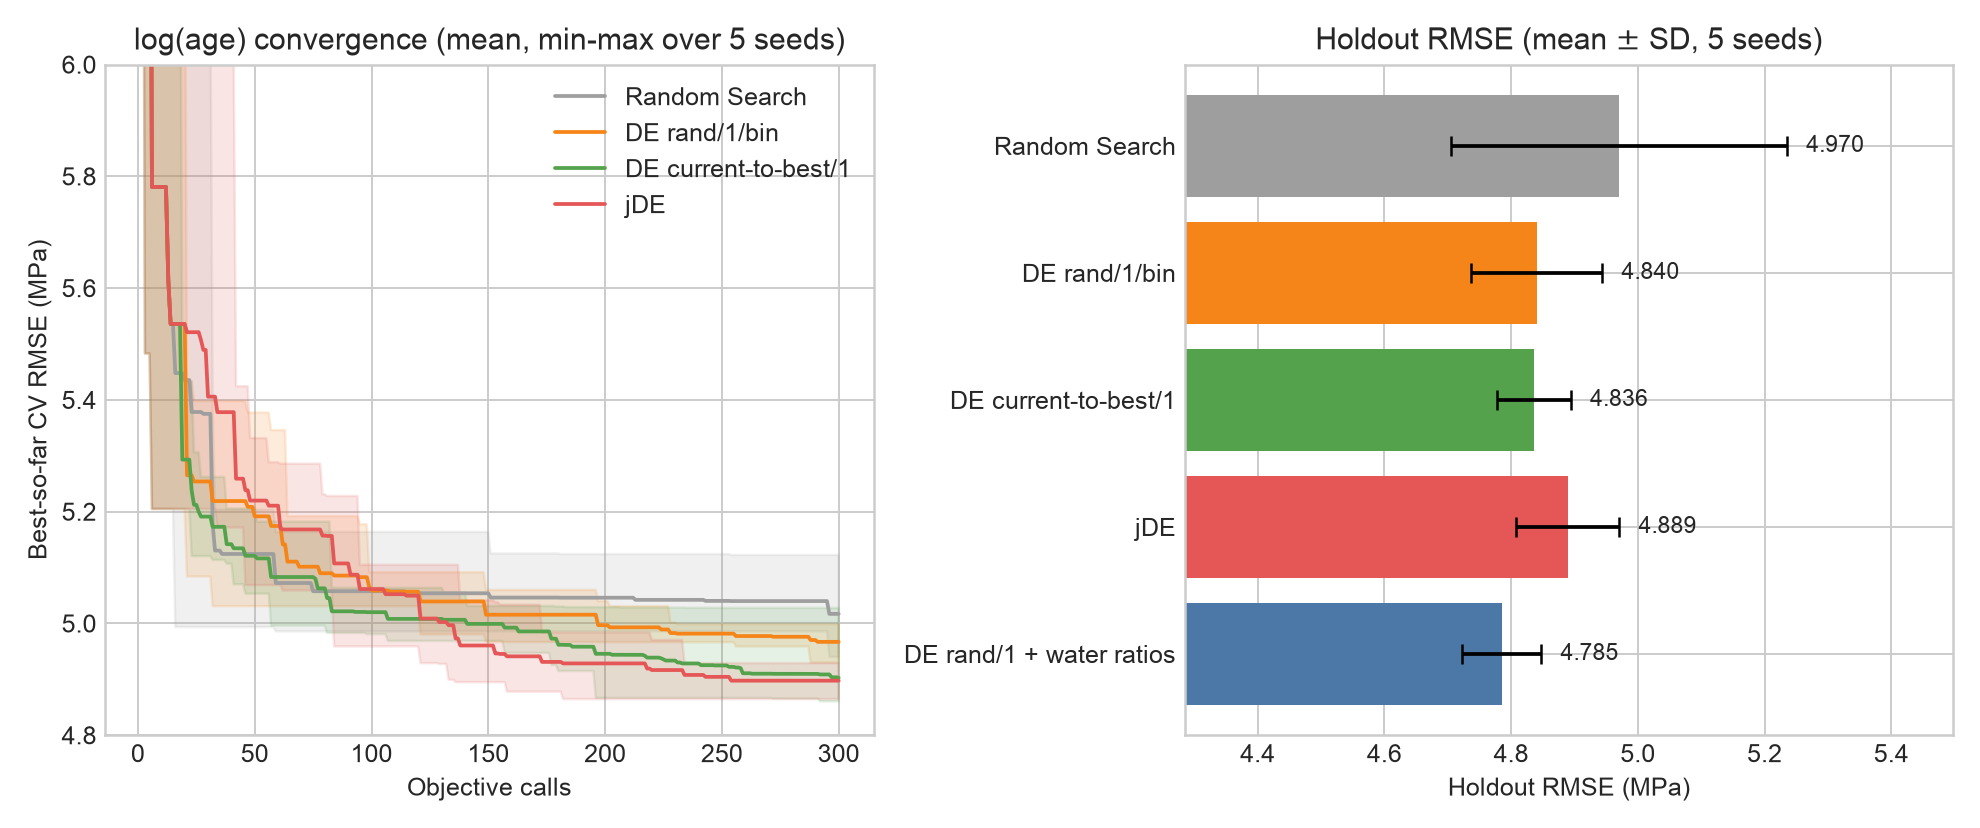
\includegraphics[width=\textwidth]{assets/de_variants.png}\caption{Left: best-so-far CV RMSE on ln(age) features (mean and min--max over five seeds). Right: holdout RMSE for the DE variants and the water-ratio feature ablation.}\label{fig:variants}\end{figure}
\subsection{Demonstration model and caveats}
By the pre-registered rule, the validation-selected demonstration is DE/current-to-best/1/bin, seed 55 (validation RMSE 4.8606 MPa; holdout RMSE 4.8672 MPa, $R^2=0.8975$). Figure~\ref{fig:extpred} shows its holdout predictions and residuals, with all points retained. The demonstration is one model chosen by validation error and should not be read as an average; the five-seed rows of Table~\ref{tab:extension} are the aggregate evidence.
\begin{figure}[htbp]\centering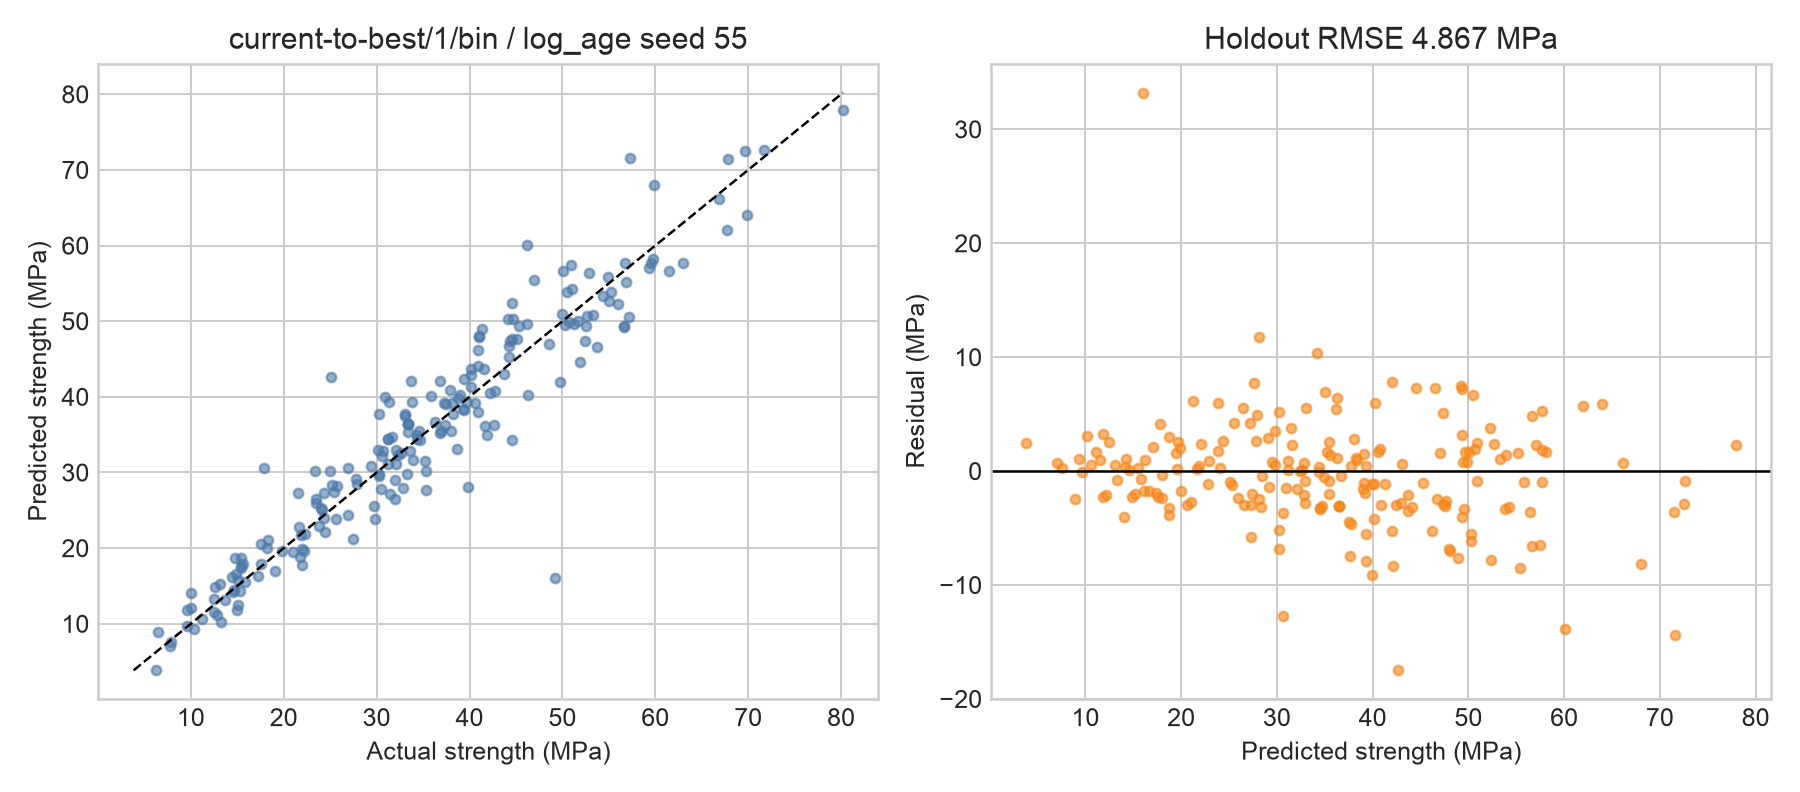
\includegraphics[width=\textwidth]{assets/extension_prediction.png}\caption{Holdout predictions and residuals for the validation-selected extension demonstration (current-to-best/1/bin, seed 55).}\label{fig:extpred}\end{figure}
The extension uses one dataset, one fixed partition and five seeds. It shows that a physically motivated input transform helps all three methods substantially; it does not show that DE outperforms Random Search or that the result transfers to other data. Section~\ref{sec:extension2} examines the DE--Random Search gap further.

\section{Extension 2: Kernel Search Space and Split Replication}\label{sec:extension2}
\subsection{Protocol}
Two follow-up questions were pre-registered in \texttt{docs/protocol-extension2.md} before any run. All settings of the earlier extension are kept (ln(age) features, fold-local scaling, bounds, DE/rand/1/bin with $F=0.8$, $CR=0.9$, seeds 11--55, selection by CV RMSE only, one holdout evaluation after all selections were frozen). The disclosures above still apply, and the holdout had in addition been seen in Extension~1.

\emph{E2a: higher-dimensional search space.} An unsaved development probe of an RBF kernel with one $\gamma$ per feature (ARD) had suggested a lower CV RMSE and contained no Random Search comparison. The ARD kernel multiplies each standardized column by $\sqrt{\gamma_j}$, giving $k(x,x')=\exp(-\sum_j\gamma_j(x_j-x'_j)^2)$, so the search space is 10-dimensional ($\log C$, $\log\epsilon$ and eight $\log\gamma_j$). Random Search and DE received the same 1{,}500-call budget (DE population 50). A shared-$\gamma$ control with the same 1{,}500 calls separates the effect of the kernel from the effect of the larger budget.

\emph{E2b: replication of the DE--Random Search comparison.} The 300-call ln(age) comparison of Extension~1 was repeated on five further group-disjoint outer splits (same sizes, \texttt{random\_state} 101--105). Splits overlap one another and the original, so they are not independent.
\subsection{ARD results}
\begin{table}[htbp]\centering\footnotesize\caption{Extension 2a: 1{,}500 calls per run, five seeds, mean $\pm$ SD. Holdout was scored once after selection.}\label{tab:ext2ard}
\begin{tabular}{llcc}\toprule
Search space & Method & Validation RMSE (MPa) & Holdout RMSE (MPa)\\\midrule
Shared $\gamma$ (3-D) & Random Search & $4.9185\pm0.0323$ & $4.8381\pm0.1064$\\
Shared $\gamma$ (3-D) & DE/rand/1/bin & $4.8581\pm0.0000$ & $4.8699\pm0.0060$\\
ARD (10-D) & Random Search & $5.1116\pm0.1766$ & $4.9693\pm0.3940$\\
ARD (10-D) & DE/rand/1/bin & $4.8811\pm0.0633$ & $4.6787\pm0.4899$\\\bottomrule
\end{tabular}\end{table}
Table~\ref{tab:ext2ard} shows three things. First, Random Search deteriorates in the 10-D space (validation 5.1116 versus 4.9185 MPa in 3-D), while DE does not (4.8811 versus 4.8581 MPa), so DE's validation advantage grows from 0.06 MPa in 3-D to 0.23 MPa under ARD. Second, the ARD kernel did not improve validation RMSE over the shared-$\gamma$ kernel: its best DE mean (4.8811 MPa) is slightly worse than the shared-$\gamma$ DE mean (4.8581 MPa), and the lower CV value suggested by the development probe was not reproduced under this protocol. Third, ARD holdout RMSE varies widely across seeds (SD 0.39--0.49 MPa); the nominally lowest ARD DE mean (4.6787 MPa) is not supported by validation and is within that spread of the other rows. With a 1{,}500-call budget the 3-D Random Search holdout (4.8381 MPa) is actually marginally below the 3-D DE holdout (4.8699 MPa), and all five 3-D DE seeds converge to the same validation optimum. No claim is made that ARD improves accuracy.
\subsection{Split replication}
\begin{table}[htbp]\centering\footnotesize\caption{Extension 2b: Random Search minus DE/rand/1/bin, mean over five seeds (positive favours DE). Split 42 is the original partition.}\label{tab:ext2rep}
\begin{tabular}{lccccc}\toprule
Split & Default SVR & RS holdout & DE holdout & $d$ holdout & $d$ validation\\\midrule
101 & 7.7818 & 4.9650 & 4.8165 & 0.1485 & 0.0766\\
102 & 7.2445 & 5.1060 & 4.8981 & 0.2079 & 0.0981\\
103 & 7.3624 & 4.7127 & 4.5541 & 0.1586 & 0.0404\\
104 & 8.4922 & 4.9841 & 5.0647 & $-0.0806$ & 0.0995\\
105 & 7.7067 & 4.6104 & 4.4654 & 0.1450 & 0.0599\\
42 (original) & 7.4780 & 4.9700 & 4.8402 & 0.1298 & 0.0501\\\bottomrule
\end{tabular}\end{table}
DE has the lower mean validation RMSE on all six splits (mean difference 0.071 MPa, approximate 95\% $t$-interval 0.045--0.097) and the lower mean holdout RMSE on five of six (mean 0.118 MPa; interval 0.012--0.224; over the five new splits alone, mean 0.116 MPa with interval $-0.024$ to 0.256, which includes zero). These intervals treat splits as independent, which they are not, and are based on six values, so they are indicative only. The evidence is consistent with a small real advantage for DE on this problem of roughly 0.1 MPa (2--3\%) in holdout RMSE, small compared with the effect of the input representation (about 1.4 MPa), and it is not a demonstration of general superiority.
